\chapter{Einleitung}\label{einleitung}
Zu Beginn soll ein kurzer Überblick über die Hintergründe und die bearbeitete Problemstellung gegeben werden.
Hierfür wird in diesem Abschnitt erläutert, wieso dieses Thema von Bedeutung ist. Außerdem wird die genaue Problemstellung erörtert und eine Abgrenzung zu verwandten Arbeiten gegeben.

\section{Motivation}\label{motivation}
Laut statistischem Bundesamt \cite{destatis} gab es im Jahr 2015 insgesamt 2.5 Millionen Verkehrsunfälle mit 3459 Todesopfern auf deutschlands Straßen zu beklagen. Damit ist die Zahl der Unfallopfer schon im zweiten Jahr in Folge angestiegen. Studien belegen, das bis zu 90\% aller Unfälle auf menschliches Versagen zurückzuführen ist \cite{Dingus08032016}. Speziell die Ablenkung durch elektronische Geräte, wie beispielsweise Smartphones, am Steuer erhöhen das Riskio eines Unfalls deutlich.
Da diese Faktoren nicht auf maschinelles Fehlverhalten zurückführen lassen können diese Unfallquellen durch autonomes Fahren verhindert werden.\\
Grundsätzlich unterscheidet man verschiedene Stufen des automatisierten Fahrens (siehe Abb. \ref{fig:autoStufe}).
Die Stufen $1$ und $2$ sind dabei das klassische Fahren ohne technische Eingriffe. Die Technik dient hier allenfalls zur Unterstützung. Stufe $3$ dagegen bietet schon Systeme an, welche von sich aus autonom in gewissen Situation fahren können, allerdings dauerhaft durch den Menschen überwacht und im Notfall übersteuert werden müssen. Der Autopilot von Tesla ist ein Beispiel für solch ein System, auch wenn der Name etwas anderes Vermuten lässt. Hochautomatisierte Fahrzeuge können in bestimmten Szenarien vollkommen ohne Überwachung agieren und erkennen ihre Systemgrenzen. Bei erreichen solch einer Grenze wird der Fahrer dazu aufgefordert zu übernehmen. Solche Systeme sind derzeit schon möglich. In Stufe $4$ wird diese Technik noch so erweitert, dass in vorgegebenen Szenarien (z.B. Autobahnfahrt) keinerlei Interaktion des Fahrers mehr von Nöten ist. Das Fahrzeug kann alle Umstände selbstständig meistern.
Die letzte Stufe und damit auch das Ziel der Forschung ist es ein System zu bauen, welches komplett fahrerlos in beliebigen Szenarien agieren kann.\\
\begin{figure}[t]\centering
  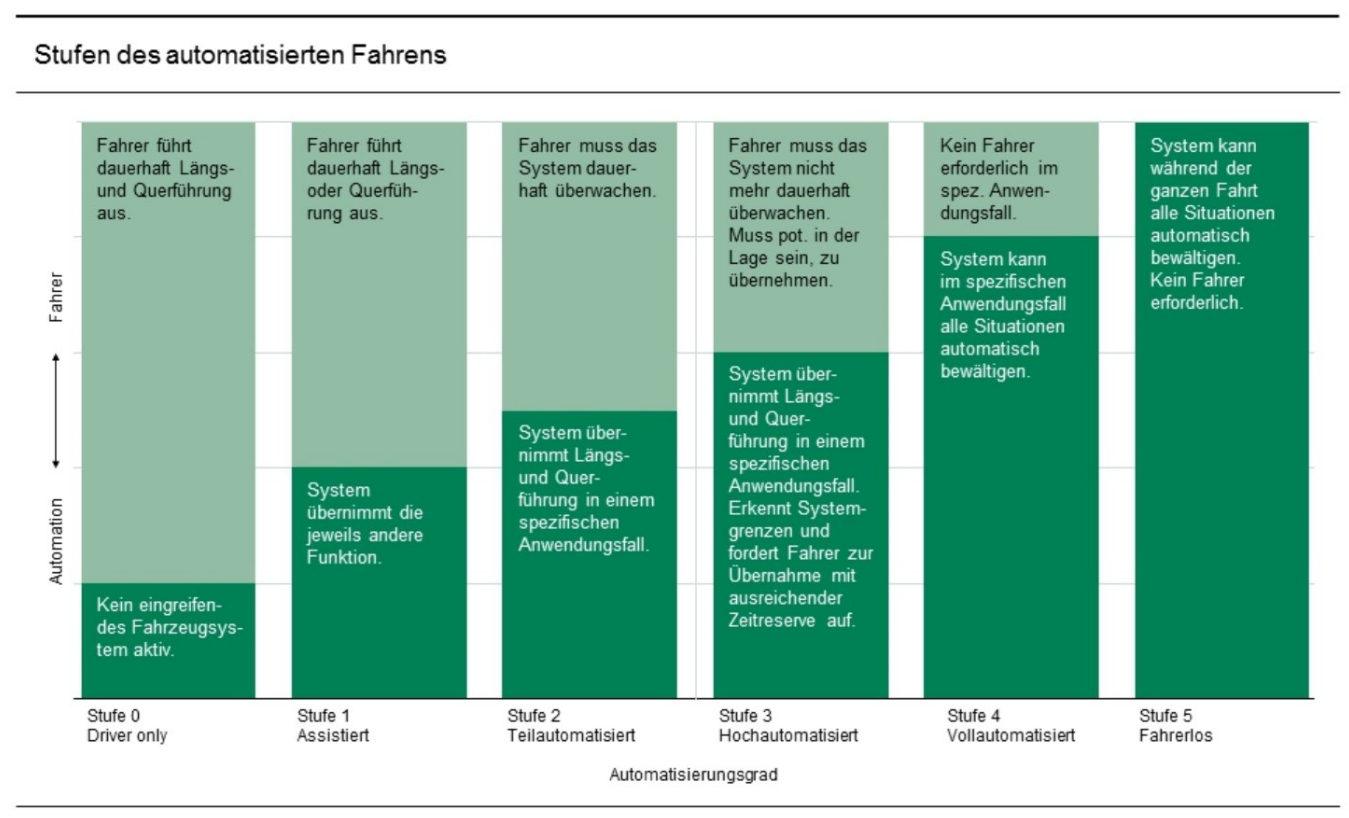
\includegraphics[width = 140mm]{bilder/stufen_snip.png}
  \caption{Stufen des automatisierten Fahrens. Aktuelle Fahrzeuge befinden sich meist in Stufe 2 oder 3. Für höhere Stufen gibt es aktuell noch keine rechtliche Grundlage und noch keine ausgereifte Technik. \cite{stufePic}}\label{fig:autoStufe}
\end{figure}
Um diese Ziel zu erreichen fließen, neben der Entwicklung von Elektroantrieben, die meisten Forschungsgelder die Entwicklung solcher Systeme. Die Wichtigkeit dieses Gebiets lässt sich daran Erkennen, dass selbst Firmen mit keinerlei Erfahrung im Automobilbereich an diesem Thema forschen und damit sogar etablierte Hersteller gefährden.
Das wichtigste für autonomes Fahren ist die genaue Kenntnis über das Fahrzeugumfeld. Es muss dem Fahrzeug zu jeder Zeit bekannt sein wo es sich befindet, wie der weitere Streckenverlauf aussieht und welche Hindernisse es evtl. in der Fahrspur gibt. Hierfür bedarf es einer Vielzahl von zusätzlichen Sensoren und Steuergeräten um all dies zuverlässig und in Echtzeit zu berechnen.
Für die Fahrspurerkennung gibt es aktuell mehrere Systeme um diese zu erkennen:\\
\begin{description}
\item[GPS und Kartenmaterial]
Mit Hilfe eines GPS-Sensors und hochgenauem Kartenmaterial kann das Fahrzeug seine genaue Position, sowie den weiteren Straßenverlauf erkennen. GPS ist allerdings nicht zu 100\% genau und kann in Tunneln oder Baustellenbereichen zu falschen Ergebnissen führen.
\item[Visuelle Erkennung der Fahrbahnmarkierungen]
Daher gibt es zusätzlich eine visuelle Erkennung der Fahrbahnmarkierungen um die Lokalisierung über GPS zu unterstützen. Dies kann über Mono- oder Stereokameras oder auch mit Hilfe eines Laserscanners erreicht werden und bietet damit eine alternative Möglichkeit die weitere Trajektorie zu planen. 
\end{description}
Leider gibt es Situationen in denen keines der beiden genannten Systeme eine zufriedenstellende Lösung anbietet. Abbildung \ref{fig:crash} zeigt eine Situation auf einer mehrspurigen Straße, auf der eine Spur durch ein havariertes Fahrzeug (rot) blockiert ist. Die beiden schwarzen Fahrzeuge haben nun die Möglichkeit auf ihrer Spur zu bleiben und anzuhalten oder auf die mittlere Spur auszuweichen. In diesem Fall würde sich die Fahrbahn mit den beiden genannten Fahrspurerkennungen auf zwei Spuren reduzieren und es könnte zum Stau kommen.
Hier kommt eine dritte Möglichkeit für die Spurerkennung ins Spiel: Die Kolonnenspurerkennung.Hinterherfahrende Fahrzeuge auf der mittleren bzw. rechten Spur beobachten das Verhalten der beiden schwarzen Fahrzeuge und erkennen ein Ausweichmanöver auf die mittlere Spur. Diese Information soll nun genutzt werden um, falls ausreichend Platz vorhanden, ebenfalls ein solches Ausweichmanöver zu fahren. Dies würde zu den drei roten Trajektorien führen. In dieser Situation wären trotz blockierter linker Spur immer noch drei Fahrspuren aktiv und die Gefahr eines Staus wäre deutlich geringer.\\
\begin{figure}[t]\centering
  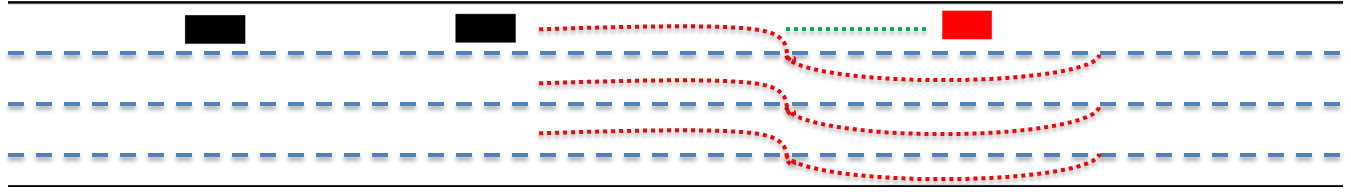
\includegraphics[width = 140mm]{bilder/Szenario_crash.png}
  \caption{Szenario einer dreispurigen Fahrbahn auf der ein Fahrzeug (rot) die linke Fahrspur blockiert. Die beiden schwarzen Fahrzeuge können entweder auf ihrer Spur bleiben und anhalten oder auf die mittlere Spur ausweichen.}\label{fig:crash}
\end{figure}
Eine solche Erkennung erfordert natürlich weitere Rechenressourcen, welche im Fahrzeug aufgrund des Bauraummangels nur begrenzt vorhanden sind und die CPUs in den ECUs nicht unendlich viel Rechenkapazität liefern. Der Trend geht deshalb hin zu hybriden Steuergeräten, also solche, die neben einer normalen CPU auch noch eine zusätzliche GPU beinhalten. Diese kann dafür verwendet werden sequentielle Rechenlast von der CPU zu nehmen und stattdessen parallele Last auf der GPU zu erzeugen. Ein Beispiel für solch ein hybrides Steuergerät ist das \textit{zfas}  \cite{zfas} von Audi, welches erstmals im neuen A8 im nächsten Jahr verbaut werden wird.

\section{Problemstellung}\label{problemstellung}
Im Rahmen dieser Arbeit soll zunächst eine sequentielle Referenzimplementierung für einen Algorithmus zur Extraktion von Kolonnenspuren erstellt werden. Dieser Algorithmus soll Laserrohdaten als Eingabe erhalten und die extrahierten Spurinformationen ausgeben. Da keine realen Laserdaten zur Verfügung stehen ist es außerdem notwendig ein System zur Simulation von Laserdaten zu entwickeln.\\
Anschließend soll der Algorithmus mit Hilfe einer eingebetteten GPU (Tegra K1) mittels CUDA parallelisiert und der SpeedUp analysiert werden.\\
Die weitere Arbeit ist wie folgt gegliedert:

\section{Verwandte Arbeiten}\label{verwandteArbeiten}
Es gibt viele Arbeiten zum Thema Spurerkennung. Dabei kann man zwischen kamerabasierten und sensorbasierten Ansätzen unterscheiden.
\cite{SASH}, \cite{SKAD} und \cite{aly08} nutzen Kamerabilder für ihre Spurextraktion, wobei \cite{SASH} die Bilder mittels Top-Hat-Transformation glättet und anschließend mit einem Region-of-interest-Ansatz mittels Vergleich mit einem Testbild die Spuren extrahiert. \cite{SKAD} dagegen verwendet einen Partikelfilter für die Spurextraktion, während \cite{aly08} eine Art Top-View aus den einzelnen Kameras zusammensetzt um anschließend in diesem Bild mittels RANSAC die Fahrbahnmarkierungen zu extrahieren.\\
\cite{JDS01} und \cite{WSD07} dagegen setzten auf Radar- und/oder Lasersensoren zur Streckenerkennung. \cite{JDS01} verwendet dabei zunächst eine punktbasierte Segmentierung der Laserdaten, ähnlich wie in dieser Arbeit, um anschließend eine ROI-Suche auf den gewonnenen Segmenten zu absolvieren um so statische Objekte (Spur) und dynamische Objekte (Verkehrsteilnehmer) zu identifizieren. In \cite{WSD07} dagegen wird eine erweiterte Belegungskarte verwendet um statische und dynamische Objekte zu trennen und so statische Straßengrenzen zu extrahieren.\\
Eine solche Belegungskarte wird in \cite{WBU13} in Intervalle gegliedert und in \cite{WBU15} dazu genutzt ein System zur Kolonnenspurerkennung zu implementieren, sehr ähnlich zur Referenzimplementierung der vorliegenden Arbeit.